\documentclass[tikz, margin=1in]{standalone}

\usetikzlibrary{calc, arrows.meta, bending}

\definecolor{mygray}{HTML}{aaaaaa}

\begin{document}
    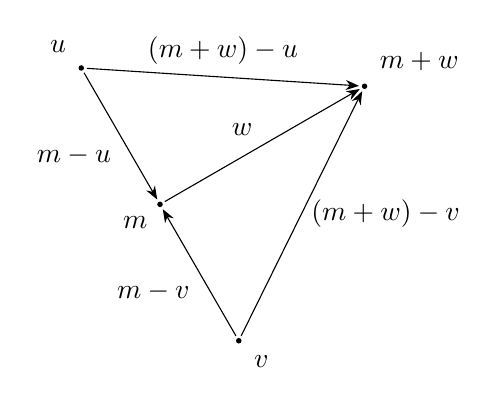
\begin{tikzpicture}[
            % color=mygray,  
            point/.style={radius=1pt},
            vec/.style={arrows=-Stealth, shorten >=2pt, shorten <=2pt}            
            ]
        \path coordinate (u) at ($(2,1) + (120:2)$)
              coordinate (v) at ($(2,1) + (300:2)$)
              coordinate (m) at ($(u)!0.5!(v)$);

        \path let \p{uv} = ($(v)-(u)$),
                  \p{uv'} = ($0.75*(\p{uv})$),
                  \p{w} = (-\y{uv'},\x{uv'}) in
              coordinate (m+w) at ($(m)+(\p{w})$);

        \fill (u) circle[point] node[above left=2pt] {\(u\)}
              (v) circle[point] node[below right=2pt] {\(v\)}
              (m) circle[point] node[below left=1pt] {\(m\)}
              (m+w) circle[point] node[above right=2pt] {\(m+w\)};

        \draw[vec] (m) to node[above left] {\(w\)} (m+w);
        \draw[vec] (u) to node[below left] {\(m-u\)} (m);
        \draw[vec] (v) to node[below left] {\(m-v\)} (m);
        \draw[vec] (u) to node[above=1pt] {\((m+w)-u\)} (m+w);
        \draw[vec] (v) to node[right] {\((m+w)-v\)} (m+w);
    \end{tikzpicture}
\end{document}